\section*{Consigna}

A continuación se muestra el comportamiento de la ventana de transmisión de un cliente al subir un archivo a un servidor:

\begin{figure}[H]
    \centering
    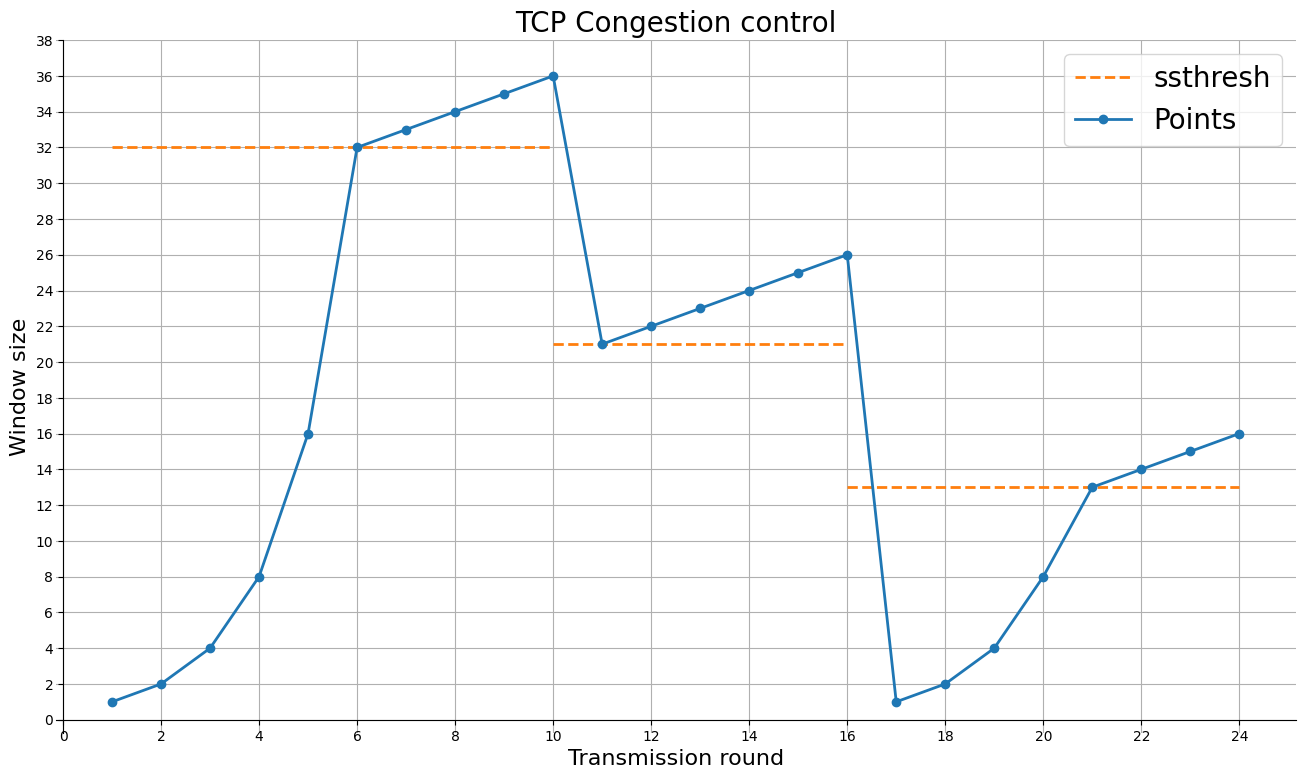
\includegraphics[width=0.95\linewidth]{Images/grafico.png}
\end{figure}

Describa el comportamiento del gráfico, mencionando el algoritmo de control de congestión utilizado, describir sus etapas, cómo se actualiza la ventana, los parámetros principales del algoritmo de congestión y el evento que causa el cambio de etapa.

\section*{Resolución}

\begin{itemize}
\item TCP Reno.
\item Slow Start.
\item Congestion avoidance.
\item Fast recovery.
\item ssthresh, cwnd.
\item Triple ACK, cada ack aumenta en uno el cwnd.
\end{itemize}


